\chapter{Theoretische Grundlagen}
In diesem Kapitel werden die für die Realisierung benötigten Technologien und
Methoden beschrieben.

Zuerst wird erläutert, was man unter einem NoSql-System versteht. Anschließend
wird die Entstehungsgeschichte der NoSql-Systeme kurz erläutert. Danach werden
die verschiedenen Arten von NoSql und speziell von Schlüssel-Wert-Systemen
beschrieben.

Danach folgt der Vergleich von Memcached, Redis und Voldemort. Dazu werden
zuerst die jeweiligen Systeme erläutert. Anschließend folgt der eigentliche
Vergleich, dazu werden die jeweiligen Eigenschaften kurz erläutert und danach
wie die jeweiligen Systeme dies umsetzen.

\section{NoSql}
NoSql-Systeme sind keine neue Erfindung, sondern entwickelten sich quasi
parallel mit den relationalen Systemen. Der Grund warum erst jetzt NoSql einen
so großen Durchbruch erfährt, hängt vor allem mit dem \gls{BigData}-Gedanken
zusammen. Vor BigData war es üblich die Geschäftsdaten auf einem
Datenbank-Server zu speichern und diesen vertikal zu skalieren, bis ein neuer
Server angeschafft wurde. Mit der Entwicklung der Sozialen-Netzwerke und der
zunehmenden Vernetzung von Alltagsgegenständen stieg die erzeugte Datenmenge
rapide auf Peta-, Exa-Byte Bereiche an. Damit war man gezwungen die Daten auf
viele Maschinen zu verteilen. Zu den Anfangszeiten versuchten die relationalen
Anbieter dies mit ihrer herkömmlichen Technologie. Allerdings scheiterten sie an
den Anforderungen. Denn sie versuchten horizontale Skalierbarkeit, Konsistenz
der Knoten und Daten, Datenreplikation, hohe Verfügbarkeit und schnelle
Antwortzeiten miteinander zu kombinieren. Dies konnte jedoch aufgrund der
Architektur der relationalen Systeme nicht funktionieren. Deshalb wurde nach
Alternativen gesucht, den NoSql-Systemen.

Was sind nun konkret NoSql-Systeme und was bedeutet NoSql eigentlich? Obwohl der
NoSql Begriff heute so eine Aktualität besitzt, gibt es keine einheitliche
Begriffsdefinition. Vielmehr ist NoSql ähnlich wie \gls{AJAX} ein Sammelbegriff
für verschiedene Technologien und Ideen. Während früher NoSql wörtlich
für \enquote{no Sql} also \enquote{kein Sql} stand steht es heute eher für
\enquote{not only Sql} also \enquote{nicht nur Sql}. Auch ab wann man ein System
als NoSql-System zählt, ist nicht klar geregelt. Vielmehr gibt es eine Reihe von
Punkten, die ein System erfüllen kann wie: \cite{Edlich2011}

\begin{itemize}
    \item Das zugrundeliegende Datenmodell ist nicht relational.
    \item Die Systeme sind von Anbeginn auf eine verteilelte und horizontale
        Skallierbarkeit ausgerichtet.
    \item Das NoSql-System ist Open-Source.
    \item Das System ist schemafrei oder hat nur schwache Schemarestriktionen.
    \item Aufgrund der verteielten Architektur unterstützt das System einfache
        Datenreplikation.
    \item Das System besitz eine einfache \gls{API}.
    \item Dem System liegt meist auch ein anderes Konsitenzmodell zugrunde:
        \gls{BASE} aber nicht \gls{ACID}.
\end{itemize}

Allerdings muss man bei NoSql gewisse Einschränkungen machen. NoSql-Systeme
verfügen zwar über die Eigenschaften Verfügbarkeit, Konsistenz der Knoten und
Partitionstoleranz, jedoch können niemals alle drei Eigenschaften gleichzeitig
erfüllt sein, sondern nur zwei. Diese Problematik ist auch unter
dem \gls{CAP}-Theorem bekannt. Deswegen gibt es auch viele verschiedene
NoSql-Systeme.

\subsection{Entwicklungsmeilensteine}
Der Ursprung von NoSql ist die im Jahr 1979 von Ken Thompson entwickelte
Datenbank DBM\footnote{\url{http://www.gnu.org/software/gdbm/gdbm.html}}, die
bis heute noch von Linux verwendet wird. Die ersten NoSql Datenbanken, die
heute noch existieren entstanden in den 80er-Jahren, wie
Lotus Note\footnote{\url{http://www-03.ibm.com/software/products/de/ibmdomino}},
BerkleyDB\footnote{\url{http://www.oracle.com/us/products/database/berkeley-db/index.html}},
GT.M\footnote{\url{https://sourceforge.net/projects/fis-gtm/https://sourceforge.net/projects/fis-gtm/}},~\dots .
Der Begriff NoSql wurde das erste Mal 1998 von Carlo Strozzi benutzt, der eine
relationale Datenbank entwickelt hatte jedoch ohne Sql. Der richtige Durchbruch
kam allerdings erst im Jahr 2000 mit dem Web 2.0 und den daraus resultierenden
Anstieg des Datenvolumens. Dieser Datenanstieg erforderte neue Methoden zur
effizienteren Speicherung und Verarbeitung. Google war dabei der Vorreiter mit
seinem Map-/Reduce-Ansatz. Die Idee dabei ist es, eine große Datenmenge in
kleinere Pakete aufzuteilen und diese dann unabhängig voneinander zu verarbeiten.
Anschließend werden die einzelnen Zwischenergebnisse gesammelt und zu einem
Gesamtergebnis zusammengefasst. Diese Idee ließ sich sehr gut mit den Ideen
der funktionalen Programmiersprachen umsetzen, denn dort wird auf einer Kopie
der tatsächlichen Daten gearbeitet. Später zogen die anderen großen Firmen mit
eigenen Lösungen nach und heute kann man sagen, dass es den Map-/Reduce-Ansatz
nicht mehr gibt, sondern verschiedene Implementierungen, die für einen gewissen
Einsatzzweck entwickelt wurden. Die Entwicklung der modernen NoSql-Systeme
begann im Jahr 2005 mit Systemen wie Neo4j\footnote{\url{http://www.neo4j.com}},
Redis, Cassandra\footnote{\url{http://cassandra.apache.org}},~\dots{} und hält bis
heute noch an.

\subsection{Arten von NoSql-Systemen}
Wie oben schon beschrieben existieren eine Vielzahl an unterschiedlichsten
NoSql"~Systemen. Dies hat zur Folge, dass es nicht leicht ist das für
seinen Anwendungsfall passende System zu finden. Deshalb kam der Gedanke
NoSql-Systeme nach bestimmten Kriterien zu sortieren um eine bessere Entscheidung
treffen zu können. Schnell entwickelten sich mehrere Kriterien. Die gröbste
Einteilung, die man vorgenommen hat, war die Einteilung in Kern-NoSql-Systeme
und Soft-NoSql-Systemen. Wobei die Grenze und der Unterschied zwischen den
Gruppen nicht klar geregelt ist. Danach werden NoSql-Systeme häufig nach ihrem
zugrundeliegenden Datenmodell eingeteilt. Nachfolgend eine Einteilung der
NoSql-Systeme nach dem Datenmodell mit einer Erklärung was man sich unter dem
jeweiligen Typ vorzustellen hat und einige Vertreter davon:

\begin{itemize}
    \item Kern-NoSql-Systeme
        \begin{description}
            \item[dokumentenbasierte Systeme] Dokumentenbasierte System
                speichern die Daten in Dateien, meist im \gls{JSON}-Format, ab.
                Zu dieser Gruppe gehören Systeme wie MongoDB oder CouchDB.
            \item[Schlüssel-Wert-Systeme] Schlüssel-Wert-Systeme speichern wie
                der Name schon sagt die Daten unter einem gewissen Schlüssel ab,
                über den dann später die Daten wieder gelesen werden. Zu dieser
                Gruppe gehören Systeme wie Redis, Voldemort, Memcached.
            \item[graphbasierte Systeme] Bei graphbasierten Systemen liegen die
                Daten als Graph vor. Solche Systeme ermöglichen es leicht
                herauszufinden, welcher Knoten mit einem anderen Knoten in
                Beziehung steht. Dies wird bei Sozialen-Netzwerken bezutzt um
                herauszufinden, wer \enquote{Freund} von jemanden ist. Zu
                dieser Gruppe gehören Systeme wie Neo4j.
            \item[spaltenorientierte Systeme] Spaltenorientierte Systeme haben
                Ähnlichkeiten mit relationalen Systemen, die ja auch über
                Spalten verfügen. Allerdings kann man bei einem
                spaltenorientierten System eine Liste von Schlüssel-Wert-Paaren
                abspeichern und im Extremfall kann sogar die Spalte eine Liste
                von Schlüssel-Wert-Paaren sein. Zu dieser Gruppe gehören Systeme
                wie HBase, Cassandra.
        \end{description}
    \item Soft-NoSql-Systeme
        \begin{description}
            \item[XML-Datenbanken] XML-Datenbanken sind spezielle
                dokumentenbasierte Systeme, bei denen statt \gls{JSON}-Dateien
                \gls{XML}-Dateien benutzt werden.
            \item[Objekt-Datenbanken] Objekt-Datenbanken speichern
                Objektstrukturen ab. Vorraussetzung ist allerdings, das die
                Objekte serialisierbar sind. Werden solche Objekt-Datenbanken
                anstelle von relationalen Datenbanken eingesetzt, dann kann man
                sich den Einsatz von \gls{ORM}-Frameworks wie
                Hibernate\footnote{\url{http://www.hibernate.org}}
                oder EclipseLink\footnote{\url{http://www.eclipse.org/eclipselink}}
                sparen.
        \end{description}
\end{itemize}

Die hier untersuchten Systeme gehören alle zu den Schlüssel-Wert-Systemen.

\section{Schlüssel-Wert-Systeme}
Schlüssel-Wert-Systeme sind Systeme, die wie der Name schon sagt, einen Wert,
also die Daten unter einem bestimmten Schlüssel ablegen. Der Zugriff auf den
abgelegten Wert erfolgt anschließend ebenfalls über den Schlüssel. Die Schlüssel
und die Werte können dabei ganz verschiedene Formen aufweisen. Die Schlüssel
sind im einfachsten Fall einfache Zeichenketten mit einer spezifischen Länge.
Andere Systeme lassen erst einmal oder mehrmals einen Hash-Algorithmus über den
Daten laufen und nehmen die erzeugte Hash-Summe als Schlüssel. Auch die Werte
sind im einfachsten Fall einfache Zeichenketten, jedoch können manche Systeme
auch komplexere Datenstrukturen wie Listen, Mengen, Wörterbücher,~\dots{}
speichern. Die Schlüssel-Wert-Systeme lassen sich nochmals in verschiedene
Gruppen einteilen, wobei jede Gruppe eine Eigenschaft fokussiert.

\subsubsection{Arten von Schlüssel-Wert-Systemen}
Schlüssel-Wert-Systeme lassen sich in Gruppen einteilen. Dabei hat jede Gruppe
eine spezifische Eigenschaft. Diese Einteilung ist aber keineswegs fest, sondern
ein System kann durchaus auch mehreren Gruppen angehören, je nachdem wie seine
aktuelle Konfiguration ist. Die folgende Liste spezifieziert die möglichen
Gruppen:

\begin{description}
    \item[Caches] \gls{RAM}-basierte Systeme oder Caches halten ihre gesamten
        Daten im \gls{RAM} vor. Deshalb werden sie oft als Zwischenspeicher
        benutzt. Dies hat zur Folge, falls ein Server ausfällt sind die Daten
        entgültig weg. Ein beliebter Anwendungsfall ist es, solch ein System
        zwischen der Anwendung und dem Datenbankserver zu schalten und die
        Ergebnisse der Datenbankanfragen für spätere Zugriffe zwischen
        zuspeichern. Zu dieser Gruppe gehören Systeme wie Memcached.
    \item[Festplatten-Systeme] Festplatten-Systeme arbeiten im Prinzip wie Caches
        nur mit der Einschränkung, dass sie ihre Daten nicht im \gls{RAM} halten
        sondern auf der Festplatte. Außerdem legen solche Systeme oft
        Wiederherstellungsdateien an. Damit sind solche Systeme gut gegen
        Ausfälle geschützt. Zu dieser Gruppe gehören Systeme wie Redis.
    \item[Sortierte Schlüssel-Wert-Systeme] Sortierte Schlüssel-Wert-System
        verfügen über Ordnungs"~ und Sortierfunktionen auf den Schlüsseln.
        Außerdem gibt es System die die Schlüssel in einer Extra Index-Tabelle
        speichern. Zu dieser Gruppe gehören Systeme wie BerkleyDB.
    \item[Eventual Consistence-Systeme] Solche Systeme stellen sicher, dass das
        System nach einer gewissen Dauer wieder in einem konsistenten Zustand
        ist. Zu dieser Gruppe gehören Systeme wie Voldemort.
\end{description}

Das erste zu untersuchende System Memcached ist ein reines Cache-System.
Redis ist ein Mischsystem aus Cache und Festplatten-System und Voldemort ist
ein Eventual-Consistence-System. Nachfolgend folgt der allgemeine Überblick über
die drei ausgewählten Systeme Memcached, Redis und Voldemort.

\subsection{Memcached}
Memcached ist ein NoSql-System und gehört in die Gruppe der
Schlüssel-Wert-Systeme und in die Untergruppe der Caches.

\foreignblockquote{english}[\cite{Memcached2017}]{Free \& open source,
high-performance, distributed memory object caching system [\ldots]}

Memcached wurde im Jahr 2003 von Brad Fitzpatrick bei der Firma Danga
Interactive heute Say Media für die Webseite LiveJournal entwickelt. Die
aktuelle Version ist die Version 1.5.0. Die ersten Versionen von Memcached
waren in Perl geschrieben. Später wurde Memcached in C neugeschrieben. Der
Vorteil von Memcached liegt in der Beschleunigung von Webseiten in dem es
Datenbank-, Webservice- und Templateergenbisse zwischenspeichert.

\foreignblockquote{english}[\cite{Memcached2017}]{[\dots{}] but intended for
use in speeding up dynamic web applications by alleviating database load.
Memcached is an in-memory key-value store for small chunks of arbitrary
data (strings, objects) from results of database calls, API calls, or page
rendering.}

Zunächst läuft auf dem Server bzw. den Servern ein oder mehrere Dienste. Der
Zugriff erfolgt dann über eine Bibliothek für die jeweilige Programmiersprache.
Die Abbildung \ref{fig:memcached-architecture} zeigt die eben beschriebene
Architektur.

Sobald Daten geschrieben oder gelesen werden sollen, berechnet die Bibliothek
aus einer mathematischen Funktion ein Ergebnis, den Hash-Wert. Dieser Wert legt
fest, welcher Server die Anfrage bekommen soll. Dieser verarbeitet dann die
Anfrage und gibt entweder die Daten zurück oder berechnet aus den zu
speichernden Daten einen weiteren Hash-Wert und speichert die Daten unter
diesem ab.

\blockquote[\cite{Schuermann2009}]{Zunächst nimmt die Client-Bibliothek den
Schlüssel und errechnet aus ihm mit einer ausgeklügelten, mathematischen
Funktion eine Zahl, den so genannten Hashwert. Diese Nummer sagt der Bibliothek,
an welchen Memcached-Daemon sie sich wenden muss. Nachdem dieser alle Daten
erhalten hat, errechnet er mit einer eigenen Hashfunktion die Speicherstelle,
unter der er die Daten schließlich einlagert.}

\begin{figure}
\centering
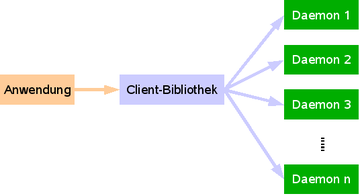
\includegraphics{images/memcached_illustration_large.png}
\caption{Architektur von Memcached \cite{Schuermann2009}}
\label{fig:memcached-architecture}
\end{figure}

Memcached hat zwei verschiedene Protokolle, welche zur Kommunikation benutzt
werden können: Text-Protokoll und Binär-Protokoll. Diese Protokolle machen
spezielle Einschränkungen auf den Schlüssel. Die maximale Schlüssellänge ist
immer 250 Zeichen lang und die Protokolle definieren, welche Zeichen erlaubt
sind als Schlüssel. Als Werte lassen sich einfache Zeichenketten oder
Binärdaten ablegen. Dies hat zur Folge, dass Memcached nicht direkt ein
Datenbankergebnis speichern kann, sondern dies erst von der Anwendung in eine
serialisierbare Struktur gepackt werden muss. Außerdem muss die Anwendung
wissen, was sich für Datentypen hinter den einzelnen Schlüssel verbergen.
Die maximale Größe ist dabei standartmäßig 64 MB, diese lässt sich allerdings
konfigurieren. Jedoch sollte die Größe immer kleiner sein als
der \gls{RAM}-Speicher des Memcached-Dienstes mit dem kleinsten
zugewiesenen \gls{RAM}.

\subsection{Redis}
Redis ist ebenfalls ein Schlüssel-Wert-System, gehört aber normalerweise in die
Untergruppe der Festplatten-Systeme. Redis lässt sich jedoch auch in die Gruppe
der Cache-Systeme eintragen, wenn eine bestimmte Konfiguration benutzt wird.
Redis wurde im Jahr 2009 von Salvatore Sanfilippo bei Redis Labs entwickelt.
Die aktuelle Version ist 4.0.1. Redis ist komplett in C geschrieben.
Der Zugriff auf einen Redis-Server erfolgt wie bei Memcached über eine
Bibliothek. Allerdings darf bei Redis im Gegensatz zu Memcached nur ein Dienst
pro Server laufen. Der wichtigste Unterschied zwischen Redis und Memcached sind
die erlaubten Schlüssel und Werte. Wie schon oben erwähnt, sind Schlüssel in
Memcached immer Zeichenketten mit einer maximalen Länge von 250 Zeichen. Im
Gegensatz dazu existiert diese Einschränkung bei Redis nicht. Dort ist es ohne
Probleme möglich, auch ein Bild als Schlüssel zu verwenden.

\foreignblockquote{english}[\cite{Redis2017}]{Redis keys are binary safe, this
means that you can use any binary sequence as a key, from a string like ‚foo‘
to the content of a JPEG file. The empty string is also a valid key. [\dots]}

Der Schlüssel wie auch die Werte dürfen lediglich die 512 MB Grenze nicht
überschreiten. Bei den zulässigen Werten unterscheidet sich Redis stark von den
anderen Systemen. Während Memcached nur Zeichenketten oder serialisierte Objekte
speichern kann ist Redis in der Lage mit Listen, Mengen und Wörterbüchern direkt
umzugehen.

\subsection{Voldemort}
Voldemort ist ein Schlüssel-Wert-System und gehört in die Untergruppe der
Eventuell-Consistence-Systeme und ist eine OpenSource Implementierung von
Amazons DynamoDB \cite{DeCandia2007}. Voldemort wurde im Jahr 2009 von Jay Kreps
und Bhupesh Bansal bei LinkedIn entwickelt. Die aktuelle Version ist 1.10.24.
Voldemort ist komplett in Java geschrieben. Der große Vorteil von Voldemort
liegt in der Verfügbarkeit. Die Idee dabei ist, falls ein Server nicht verfügbar
ist und man deswegen nicht auf die Daten zugreifen kann, dass man dann nicht
alle Server nach den Daten durchsucht, sondern nur die nächsten. Dafür werden die
Server gedanklich zu einem Ring zusammengefügt. Der Zugriff erfolgt wie bei den
anderen Systemen über eine Bibliothek. Die Abbildung \ref{fig:voldemort-logical-architecture}
zeigt exemplarisch die Verbindung eines Voldemort-Clients mit einem
Voldemort-Server. Die oberen drei Schichten stellen die Bibliothek dar, welche
von den Anwendungen benutzt wird. Die letzte Schicht stellt das eigentliche
Speichermedium dar. Die übrigen zwei Schichten stellen einen Voldemort-Server
dar. Ähnlich wie bei Memcached kann auch bei Voldemort ein oder mehrere Dienste
gleichzeitig laufen. Voldemort macht bei der Wahl der Schlüssel
und Werte keine Einschränkung. Es muss lediglich eine Klasse geschrieben werden,
die Schlüssel und die Werte serialisieren und de-serialisieren kann.

\begin{figure}
\centering
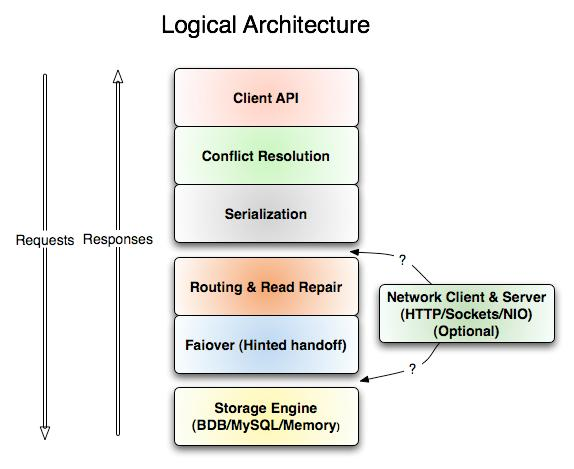
\includegraphics[scale=0.5]{images/voldemort-architecture.jpeg}
\caption{Logische Architektur eines Voldemort-Clients mit einem Voldemort-Server \cite{Voldemort2017}}
\label{fig:voldemort-logical-architecture}
\end{figure}

\section{Verteiltes System/Cluster-Bildung}
NoSql-Systeme sind wie oben schon erwähnt dafür ausgelegt, horizontal zu
skalieren. Dort werden also eher zusätzliche Server mit weniger Ressourcen
angeschafft, als bestehende Server zu erweitern, um eine gemeinsame Aufgabe zu
erfüllen. Solche Systeme werden auch verteilte Systeme oder Cluster genannt.

\blockquote[\cite{Distener2012}]{Ein verteiltes System besteht aus unabhängigen,
über ein Rechnernetz kommunizierenden Rechnern, wobei keine zentrale
Systemsteuerung existiert und der Verteilungsaspekt für alle Benutzer des
Systems möglichst transparent ist.}

Der Unterschied zwischen einem verteilten System und einem Cluster
ist dabei nicht klar definiert.

Verteilte System lassen sich in zwei Kommunikationsmodelle einteilen
Client-Server und Peer-To-Peer. Bei Client-Server stellen ein oder mehrere
Server einen Dienst bereit und die Clients wollen diesen Dienst nutzen. Dabei
haben, die einzelnen Server keine Information über die anderen Server. Eine
Sonderform von Client-Server ist das Master-Slave-Prinzip. Master-Slave ist ein
Zusammenschluss von mindestens zwei Rechnern. Ein Rechner ist dabei der Master
und nimmt alle Anfragen der Clients entgegen und verteilt diese an seine
Slaves. Somit sind die Master nach außen hin Server und nach innen auch Clients
und die Slaves sind nur Server.

Im Gegensatz dazu ist bei Peer-To-Peer die Aufteilung in Client und Server
nicht klar, denn ein einzelner Rechner kann sowohl Client als auch Server sein.
Des Weiteren haben die einzelnen Rechner Informationen über die anderen Rechner.
Werden mehrere Master-Slave-Systeme zu einem Peer-To-Peer kombiniert entsteht
ein Master-Master-Netz. Die Clients senden ihre Anfrage an einen beliebigen
Master, der die Anfrage entweder selbst beantwortet oder diese weiterleitet.

\subsection{Memcached}
Memcached ist ein klassisches Client-Server-System. Die Anwendungen, welche über
eine Bibliothek auf einen Memcached-Dienst zugreifen sind die Clients und die
Memcached-Dienste sind die Server. Die verschiedenen Memcached-Dienste haben
dabei keine Information über andere Dienste, sondern nur die Bibliothek hat
diese Information.

\foreignblockquote{english}[\cite{Memcached2017}]{The servers understand how
store and fetch items. They also manage when to evict or reuse memory. Servers
are Disconnected From Each Other Memcached servers are unaware of each other.
There is no crosstalk, no syncronization, no broadcasting, no replication.}

Falls man doch Replikation und andere Funktionen benötigt muss dies die
Bibliothek leisten oder eine andere Bibliothek.

\subsection{Redis}
Redis ist wie Memcached ein klassisches Client-Server-System. Die Anwendungen,
welche über eine Bibliothek auf den Redis-Dienst zugreifen sind die Clients und
die Redis-Dienste sind die Server. Redis lässt sich nun je nach Anforderung
konfigurieren. Im einfachsten Fall haben die verschieden Redis-Server keine
Informationen über die anderen Server. Hier muss wie bei Memcached die
Bibliothek die zusätzliche Funktionalität bereitstellen, wie die Verbindung zu
mehreren Redis-Diensten.

Eine etwas verbesserte Konfiguration ist mehrere Server im Master-Slave-Modus
zu betreiben. Dadurch ist sichergestellt, dass sowohl Master als auch die
Slaves, die gleichen Daten haben, und eine Datenwiederherstellung möglich ist.
Jedoch muss die Bibliothek immer noch den Verbindungsaufbau übernehmen und auch
solche Sachen wie, dass nur auf dem Master geschrieben und von den Slaves nur
gelesen werden darf. Dies war bis Redis 3.0 die Standardkonfiguration.

Ab Redis 3.0 ist es möglich, einen echten Cluster mit Master-Master-Replikation
zu betreiben. Für solch eine Konfiguration werden laut der offiziellen
Dokumentation 6-Server benötigt 3-Master mit jeweils 1-Slave.

\foreignblockquote{english}[\cite{Redis2017}]{Note that the minimal cluster
that works as expected requires to contain at least three master nodes. For your
first tests it is strongly suggested to start a six nodes cluster with three
masters and three slaves.}

\subsection{Voldemort}
Voldemort ist im Gegensatz zu den beiden anderen Systemen ein
Peer-To-Peer-Netzwerk. Alle beteiligten Server haben die Information, welche
anderen Server noch Teil des Clusters sind. Im Gegensatz zu Memcached und Redis
sind bei Voldemort die Server in der Lage, die Daten automatisch zu
partitionieren und zu replizieren. Dadurch ist es möglich, dynamisch auf
geplante und ungeplante Ausfälle zu reagieren. Dabei ist der Punkt zu beachten,
dass dies nur für den Initialen-Cluster funktioniert. Wenn sich die
Cluster-Struktur ändert, weil ein gänzlich neuer Server hinzugefügt wird, dann
funktioniert die automatische Replikation und Partitionierung nicht mehr,
sondern die neue Konfiguration muss erst auf alle Knoten neu verteilt werden.
Bei Voldemort muss die Bibliothek auch nicht mehr alle Server kennen, sondern es
reicht ein Server aus, von dem sich die Bibliothek, dann die
Cluster-Konfiguration holen kann.

\section{Persistenz}
Persistenz ist die Eigenschaft Objekte, Daten, logische Verbindungen,~\dots{}
über die Laufzeit der Anwendung hinaus verfügbar zu machen. Dies ist gerade
wichtig, falls es zu einem geplanten oder ungeplanten Ausfall kommt, um die
Daten wiederherzustellen.

Bei einem einzelnen Server ist dies einfach, entweder das System unterstützt
Persistenz oder eben nicht. Sobald aber mehr als ein Server im Einsatz ist wie
bei NoSql-Systemen, wo Server dynamisch hinzugefügt oder entfernt werden können,
spielt die Architektur des Systems eine Rolle. Denn dort kann entweder keine
Persistenz sein, ein einzelner Server sichert die Daten, einige Server sichern
ihre Daten oder alle Server sichern ihre Daten.

Eng mit dem Begriff der Persistenz verknüpft ist die Konsistenz. Gerade wenn
ein Server einen anderen über neue Änderungen informiert, kann es zu
Inkonsistenzen kommen.

\subsection{Memcached}
Memcached stellt selbst keine Persistenz zur Verfügung. Wenn ein oder mehrere
Server geplant oder ungeplant ausfallen, dann sind die Daten die aktuell im
\gls{RAM} waren verloren. Die Daten lassen sich auch nicht von anderen Server
holen, da immer nur ein Server die speziellen Daten speichert und wie oben
erwähnt, auch keine Kommunikation zwischen den einzelnen Memcached-Diensten
existiert.

\subsection{Redis}
Redis kann mit Persistenz oder ohne betrieben werden. Wenn man Redis ohne
Persistenz betreibt, hat man ein besseres Memcached-System.

\foreignblockquote{english}[\cite{Redis2017}]{If you wish, you can
disable persistence at all, if you want your data to just exist as long as the
server is running.}

Standardmäßig wird Redis immer mit Persistenz betrieben. Redis bietet dabei
zwei Persistenzmethoden an, welche auch zusammen benutzt werden können. Diese
beiden Methoden sind \gls{RDB} und \gls{AOF}.

\foreignblockquote{english}[\cite{Redis2017}]{It is possible to combine both
AOF and RDB in the same instance. Notice that, in this case, when Redis
restarts the AOF file will be used to reconstruct the original dataset since it
is guaranteed to be the most complete.}

Bei \gls{RDB} werden die Daten aus dem \gls{RAM} in regelmäßigen Abständen als
Zwischenstand auf die Festplatte geschrieben.

\foreignblockquote{english}[\cite{Redis2017}]{The RDB persistence performs
point-in-time snapshots of your dataset at specified intervals.}

Im Gegenzug wird bei \gls{AOF} jede Änderung in einer Datei angehängt und ein
separater Thread liest die Datei ein und schreibt die Änderungen auf die
Festplatte.

\foreignblockquote{english}[\cite{Redis2017}]{The AOF persistence logs every
write operation received by the server, that will be played again at server
startup, reconstructing the original dataset. Commands are logged using the same
format as the Redis protocol itself, in an append-only fashion.}

\subsection{Voldemort}
Voldemort kann nur mit Persistenz betrieben werden. Während bei Redis die Daten
in eine Datei geschrieben werden, verfügt Voldemort über eine Persistenz-Sicht,
die sich mit unterschiedlichen Speicher-Modellen betreiben lässt. Standardmäßig
speichert Voldemort seine Daten in eine Berkley Datenbank. Alternative lässt
sich die BerkleyDB auch durch MySql/MariaDB ersetzen. Zum testen ist es auch
möglich, die Daten lediglich im \gls{RAM} wie bei Memcached zu speichern oder
die Implementierung von Voldemort zu benutzen. Falls man mit den vorhanden
Modellen nicht zufrieden ist, kann man auch eine eigene Lösung implementieren.

\foreignblockquote{english}[\cite{Voldemort2017}]{We support a simple api for
persistence and use BDB Java edition as the default. Other storage engines
supported are MySQL, in-memory storage ( used for unit testing ) and our own
custom read-only storage engine ( generated offline as a batch process in
Hadoop ). To add a new persistence implementation you need to implements put,
get, and delete, plus provide an iterator over the values in the local store.}

Bei einem Ausfall eines Servers werden zuerst die Daten aus der Persistenz
geladen. Danach werden die aktuellsten Daten von den benachbarten Server
kopiert.
